%%%%%%%%%% DOCUMENT STUFF %%%%%%%%%%

\documentclass[10.5pt,letterpaper]{article}
\usepackage{mathtools}
\usepackage{amsmath}
\usepackage{amssymb}
\usepackage{datetime}
\usepackage{setspace}
\usepackage{tikz}
\usepackage[margin=1in]{geometry}
\usepackage{courier}
\usepackage{listings}
\usepackage{mips}
\usepackage{graphicx}
\usepackage{enumitem}
\usepackage{pgfplots}

%%%%%%%%%% FORMATTING %%%%%%%%%%

\newdate{date}{20}{07}{2017}
\spacing{1.5}
\date{\displaydate{date}}
\setcounter{secnumdepth}{0}
\newcommand\tab[1][0.5cm]{\hspace*{#1}}
\newcommand*\circled[1]{\tikz[baseline=(char.base)]{
            \node[shape=circle,draw,inner sep=2pt] (char) {#1};}}
\lstset{language=[mips]Assembler}
\usetikzlibrary{arrows,shapes,automata,petri,positioning,calc}

\tikzset{
    place/.style={
        circle,
        thick,
        draw=black,
        minimum size=6mm,
    },
        state/.style={
        circle,
        thick,
        draw=black!75,
        %fill=blue!20,
        minimum size=6mm,
    },
}

\graphicspath{{images/}}

%%%%%%%%%% CONTENT %%%%%%%%%%

%%%%% COVER PAGE %%%%%

\begin{document}
\title{CS 181: Homework 1}
\author{
	Jonathan Woong\\
	804205763\\
	Summer 2017\\
	Discussion 1A}
\maketitle
\pagebreak

%%%%% PROBLEMS %%%%%

\begin{enumerate}[label=\textbf{Problem \arabic*.}]
\item Given NFA $N$
	\begin{center}
		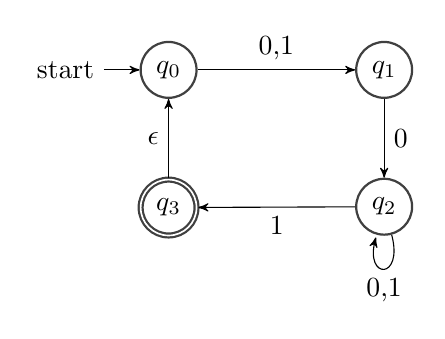
\begin{tikzpicture}[node distance=1cm and 2cm,>=stealth',auto, every place/.style={draw}]
	    \node [state,initial] (start) {$q_0$};
	    \node [state] (top-right) [right=of start] {$q_1$};
	    \node [state] (bottom-right) [below=of top-right] {$q_2$};
	    \node [state,accepting] (bottom-left) [below=of start] {$q_3$};
	    \path [->]
	    (start) edge  node {0,1} (top-right)
	    (top-right) edge node {0} (bottom-right)
	    (bottom-right) edge node {1} (bottom-left)
	    edge [loop below] node {0,1} ()
	    (bottom-left) edge node {$\epsilon$} (start);  
	\end{tikzpicture}
	\end{center}
find the language L($N$) and build DFA $DN$ equivalent to $N$.
\[\begin{tabular} {|c|c|}
\hline
state & $\epsilon$-closure \\
\hline
\{$\emptyset$\} & \{$\emptyset$\} \\
\hline
\{$q_0$\} & \{$q_0$\} \\
\hline
\{$q_1$\} & \{$q_1$\} \\
\hline
\{$q_2$\} & \{$q_2$\} \\
\hline
\{$q_3$\} & \{$q_0,q_3$\} \\
\hline
\{$q_0,q_1$\} & \{$q_0,q_1$\} \\
\hline
\{$q_0,q_2$\} & \{$q_0,q_2$\} \\
\hline
\{$q_0,q_3$\} & \{$q_0,q_3$\} \\
\hline
\{$q_1,q_2$\} & \{$q_1,q_2$\} \\
\hline
\{$q_1,q_3$\} & \{$q_0,q_1,q_3$\} \\
\hline
\{$q_2,q_3$\} & \{$q_0,q_2,q_3$\} \\
\hline
\{$q_0,q_1,q_2$\} & \{$q_0,q_1,q_2$\} \\
\hline
\{$q_0,q_1,q_3$\} & \{$q_0,q_1,q_3$\} \\
\hline
\{$q_0,q_2,q_3$\} & \{$q_0,q_2,q_3$\} \\
\hline
\{$q_1,q_2,q_3$\} & \{$q_0,q_1,q_2,q_3$\} \\
\hline
\{$q_0,q_1,q_2,q_3$\} & \{$q_0,q_1,q_2,q_3$\} \\
\hline
\end{tabular}\]
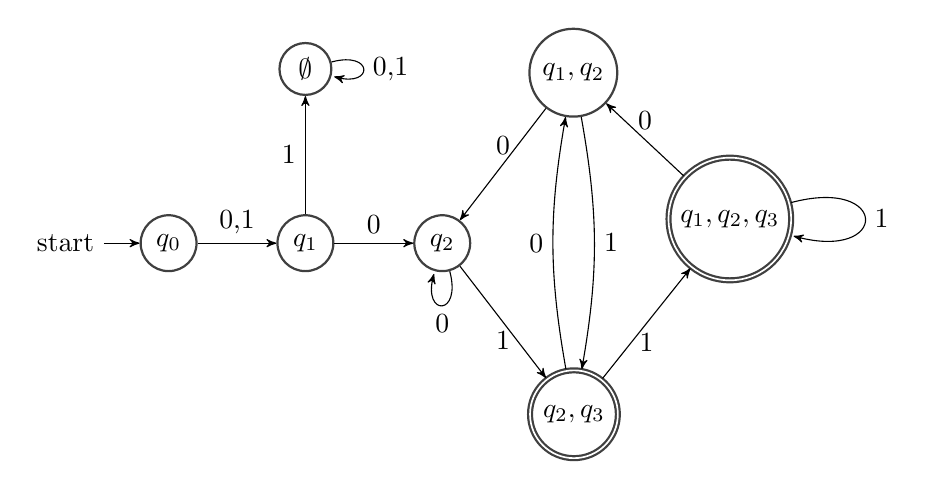
\begin{tikzpicture}[node distance=1.5cm and 1cm,>=stealth',auto, every place/.style={draw}]
	\node [state,initial] (q_0) {$q_0$};
	\node [state] (q_1) [right=of q_0] {$q_1$};
	\node [state] (q_2) [right=of q_1] {$q_2$};
	\node [state,accepting] (q_23) [below right=of q_2] {$q_2,q_3$};
	\node [state] (q_12) [above right=of q_2] {$q_1,q_2$};
	\node [state,accepting] (q_123) [above right=of q_23] {$q_1,q_2,q_3$};
	\node [state] (empty) [above=of q_1] {$\emptyset$};
	\path [->]
	    (q_0) edge  node {0,1} (q_1)
	    (q_1) edge node {0} (q_2)
	    edge node {1} (empty)
	    (q_2) edge node [below] {1} (q_23)
	    edge [loop below] node {0} ()
	    (q_23) edge node [below] {1} (q_123)
	    edge [bend left=10] node {0} (q_12)
		(q_12) edge node [above] {0} (q_2)
	    edge [bend left=10] node {1}  (q_23)
	    (q_123) edge node [above] {0} (q_12)
	    edge [loop right] node {1} ()
	    (empty) edge [loop right] node {0,1} ();  
\end{tikzpicture}
\[\boxed{\text{L}(N)=\bigg[(0 \cup 1) 0 (0 \cup 1)^*1\bigg]\cup\bigg[(0\cup1) 0 (0\cup1)^*1\bigg]^*}\]
\item Build DFA $D$ and NFA $N$ such that L($D$)=L($N$), which consists of all binary strings that have substring 00110001.
\[\Sigma = \{0,1\}\]
\[\text{L}(D)=\{x00110001y \ | \ x,y \in \Sigma^*\}\]
\[\text{DFA}\]

\begin{tikzpicture}[transform canvas={scale=0.9},node distance=1.5cm and 1cm,>=stealth',auto, every place/.style={draw}]
	\node [state,initial] (start) {};
	\node [state] (0) [right=of start] {0};
	\node [state] (00) [right=of 0] {00};
	\node [state] (001) [right=of 00] {001};
	\node [state] (0011) [right=of 001] {0011};
	\node [state] (00110) [right=of 0011] {00110};
	\node [state] (001100) [right=of 00110] {001100};
	\node [state] (0011000) [right=of 001100] {0011000};
	\node [state,accepting] (00110001) [right=of 0011000] {00110001};
	\path [->]
	    (start) edge node {0} (0)
	    edge [loop above] node {1} ()
	    (0) edge node {0} (00)
	    edge [bend left=30] node {1} (start)
	    (00) edge node {1} (001)
	    edge [loop above] node {0} ()
	    (001) edge node {1} (0011)
	    edge [bend left=30] node {0} (0)
	    (0011) edge node {0} (00110)
	    edge [bend left=45] node {1} (start)
	    (00110) edge node {0} (001100)
	    edge [bend left=60] node {1} (start)
	    (001100) edge node {0} (0011000)
	    edge [bend left=75] node {1} (start)
	    (0011000) edge node {1} (00110001)
	    edge [bend left=45] node {0} (00)
	    (00110001) edge [loop right] node {0,1} ();
\end{tikzpicture}\\\\\\\\\\\\\\
\[\text{NFA}\]

\begin{tikzpicture}[transform canvas={scale=0.9},node distance=1.5cm and 1cm,>=stealth',auto, every place/.style={draw}]
	\node [state,initial] (start) {};
	\node [state] (0) [right=of start] {0};
	\node [state] (00) [right=of 0] {00};
	\node [state] (001) [right=of 00] {001};
	\node [state] (0011) [right=of 001] {0011};
	\node [state] (00110) [right=of 0011] {00110};
	\node [state] (001100) [right=of 00110] {001100};
	\node [state] (0011000) [right=of 001100] {0011000};
	\node [state,accepting] (00110001) [right=of 0011000] {00110001};
	\path [->]
	    (start) edge node {0} (0)
	    edge [loop above] node {0,1} ()
	    (0) edge node {0} (00)
	    edge [bend left=30] node {1} (start)
	    (00) edge node {0,1} (001)
	    edge [loop above] node {0} ()
	    (001) edge node {1} (0011)
	    edge [bend left=30] node {0} (0)
	    (0011) edge node {0} (00110)
	    edge [bend left=45] node {0,1} (start)
	    (00110) edge node {0} (001100)
	    edge [bend left=60] node {0,1} (start)
	    (001100) edge node {0} (0011000)
	    edge [bend left=75] node {0,1} (start)
	    (0011000) edge node {1} (00110001)
	    edge [bend left=45] node {0} (00)
	    (00110001) edge [loop right] node {0,1} ();
\end{tikzpicture}
\pagebreak
\item Find if the language $L=\{a^3b \ ; \ a,b \in \Sigma\}$ is regular and prove that your answer is correct.\\
The language $L$ is regular because we can construct the following finite automata:\\
\begin{center}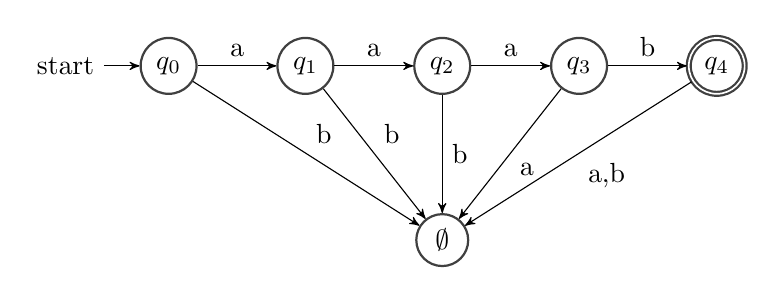
\begin{tikzpicture}[node distance=1.5cm and 1cm,>=stealth',auto, every place/.style={draw}]
	\node [state,initial] (start) {$q_0$};
	\node [state] (1) [right=of start] {$q_1$};
	\node [state] (2) [right=of 1] {$q_2$};
	\node [state] (3) [right=of 2] {$q_3$};
	\node [state,accepting] (4) [right=of 3] {$q_4$};
	\node [state] (empty) [below=of 2] {$\emptyset$};
	\path [->]
	    (start) edge node {a} (1)
	    edge node {b} (empty)
	    (1) edge node {a} (2)
	    edge node {b} (empty)
	    (2) edge node {a} (3)
	    edge node {b} (empty)
	    (3) edge node {b} (4)
	    edge node {a} (empty)
	    (4) edge node {a,b} (empty);
\end{tikzpicture}\end{center}
Here, the word $aaab$ is accepted by language $L$, and by definition, any language that is accepted by a finite automata (DFA or NFA) is also a regular language (Kleene-Myhill Theorem).
\end{enumerate}
\end{document}